% Template for ICASSP-2021 paper; to be used with:
%          spconf.sty  - ICASSP/ICIP LaTeX style file, and
%          IEEEbib.bst - IEEE bibliography style file.
% --------------------------------------------------------------------------
\documentclass{article}
\usepackage{spconf,amsmath,graphicx}
\usepackage{subcaption}

\usepackage{amsfonts}
\usepackage{amsmath}
\usepackage{amssymb}

\usepackage{amsthm}
\newtheorem{definition}{Definition}
\newtheorem{proposition}{Proposition}

\usepackage{algorithm}
\usepackage{algorithmicx}

\DeclareMathOperator{\Unif}{Unif}

\usepackage{hyperref}


% Title.
% ------
\title{Multi-target detection with the generalized method of moments}
%
% Single address.
% ---------------
\name{Author(s) Name(s)\thanks{Thanks to XYZ agency for funding.}}
\address{School of Electrical Engineering, Tel Aviv University, Tel Aviv, Israel}
%
% For example:
% ------------
%\address{School\\
%	Department\\
%	Address}
%
% Two addresses (uncomment and modify for two-address case).
% ----------------------------------------------------------
%\twoauthors
%  {A. Author-one, B. Author-two\sthanks{Thanks to XYZ agency for funding.}}
%	{School A-B\\
%	Department A-B\\
%	Address A-B}
%  {C. Author-three, D. Author-four\sthanks{The fourth author performed the work
%	while at ...}}
%	{School C-D\\
%	Department C-D\\
%	Address C-D}
%
\begin{document}
%\ninept
%
\maketitle
%
\begin{abstract}
The abstract should appear at the top of the left-hand column of text, about
0.5 inch (12 mm) below the title area and no more than 3.125 inches (80 mm) in
length.  Leave a 0.5 inch (12 mm) space between the end of the abstract and the
beginning of the main text.  The abstract should contain about 100 to 150
words, and should be identical to the abstract text submitted electronically
along with the paper cover sheet.  All manuscripts must be in English, printed
in black ink.
\end{abstract}
%
\begin{keywords}
One, two, three, four, five
\end{keywords}
%
\section{Introduction}
\label{sec:intro}

We study the multi-target detection (MTD) problem of estimating a target signal~\mbox{$x: \{0, \ldots, L-1\} \rightarrow \mathbb{R}$} from a noisy measurement that contains multiple copies of the signal, each randomly translated~\cite{bendory2019multi}, \cite{lan2020multi}, \cite{marshall2020image}, \cite{bendory2021multi}, \cite{kreymer2021two}, \cite{bendory2018toward}. Specifically, let~\mbox{$y: \{0, \ldots, N-1\} \rightarrow \mathbb{R}$} be a measurement of the form
\begin{equation}
\label{eq:model}
y[\ell] = \sum_{i=1}^{p} x[\ell - \ell_i] + \varepsilon[\ell],
\end{equation}
where \mbox{$\{\ell_i\}_{i=1}^{p} \in \{L + 1, \ldots, N-L\}$} are arbitrary translations, and~$\varepsilon[\ell]$ is i.i.d. Gaussian noise with zero mean and \mbox{variance~$\sigma^2$}.

The translations and the number of occurrences of~$x$ in~$y$ are unknown. Figure~\ref{fig:measurements} presents an example of a measurement~$y$ at different signal-to-noise ratios (SNRs). We define~\mbox{$\text{SNR} := \frac{\|x\|_\text{F}^2}{L \sigma^2}$}, where~$L$ is the length of~$x$ (in pixels), and~$\sigma^2$ is the noise variance.

\begin{figure}[!tb]
	\begin{subfigure}[ht]{0.30\columnwidth}
		\centering
		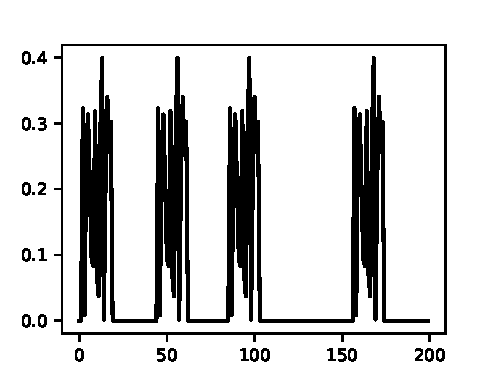
\includegraphics[width=\columnwidth]{figures/y_clean.pdf}
		\caption{No noise.}
	\end{subfigure}
	\hfill
	\begin{subfigure}[ht]{0.30\columnwidth}
		\centering
		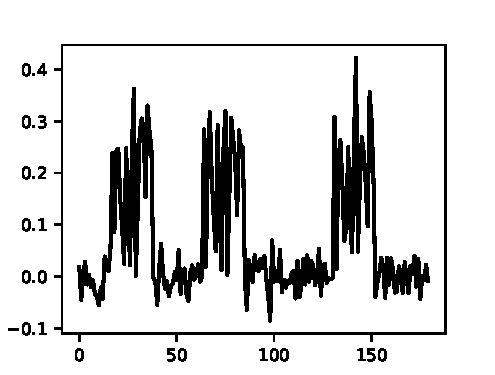
\includegraphics[width=\columnwidth]{figures/y_SNR50.pdf}
		\caption{$\text{SNR} = 50$.}
	\end{subfigure}
	\hfill
	\begin{subfigure}[ht]{0.30\columnwidth}
		\centering
		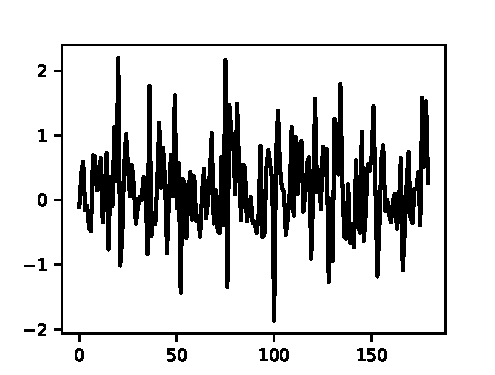
\includegraphics[width=\columnwidth]{figures/y_SNR01.pdf}
		\caption{$\text{SNR} = 0.1$.}
	\end{subfigure}
	\caption{Three measurements~$y$ from~(\ref{eq:model}) at different noise levels: no noise (left);~\mbox{$\text{SNR} = 50$} (middle);~\mbox{$\text{SNR} = 0.1$} (right). Each measurement contains multiple copies of the target signal in arbitrary locations. In this work, our goal is to estimate the target signal directly from~$y$. We focus on the low SNR regime~(e.g., panel~(c)) in which the signal occurrences are swamped by the noise, and the locations of the signal occurrences cannot be detected reliably.}
\label{fig:measurements}
\end{figure}

The MTD model arises in several scientific applications, such as passive radar~\cite{gogineni2017passive}, astronomy~\cite{schulz1993multiframe}, motion deblurring~\cite{levin2006blind}, and system identification~\cite{abed1997blind}. In particular, it serves as mathematical abstraction of the cryo-electron microscopy~(\mbox{cryo-EM}) technology for macromolecular structure determination~\cite{henderson1995potential},~\cite{nogales2016development},~\cite{bai2015cryo}. In a \mbox{cryo-EM} experiment \cite{frank2006three}, biological macromolecules suspended in a liquid solution are rapidly frozen into a thin ice layer. An electron beam then passes through the sample, and a two-dimensional tomographic projection is recorded. Importantly, the \mbox{2-D} location and \mbox{3-D} orientation of particles within the ice are random and unknown. This measurement, called \textit{micrograph}, is affected by high noise levels and the optical configuration of the microscope. This transformation is typically modeled as a convolution of the model~(\ref{eq:model}) with a point spread function, whose Fourier transform is called contrast transfer function~(CTF)~\cite{heimowitz2020reducing}, \cite{erickson1971measurement}.

In the current analysis workflow of \mbox{cryo-EM} data \cite{bendory2020single}, \cite{scheres2012relion}, \cite{punjani2017cryosparc}, the~\mbox{2-D} projections are first detected and extracted from the micrograph, and later rotationally and translationally aligned to reconstruct the~\mbox{3-D} molecular structure. This approach fails for small molecules, which induce low contrast, and thus low SNR. This makes them difficult to detect and align~\cite{bendory2018toward}, \cite{henderson1995potential}, \cite{bendory2020single}, \cite{aguerrebere2016fundamental}, rendering current \mbox{cryo-EM} algorithmic pipeline ineffective. For example, in the limit~\mbox{$\text{SNR} \rightarrow 0$}, reliable detection of signals' locations within the measurement is impossible~\cite[Proposition~3.1]{bendory2018toward}.

The MTD model was devised in \cite{bendory2018toward} in order to study the recovery of small molecules directly from the micrograph, below the current detection limit of \mbox{cryo-EM}~\cite{henderson1995potential},~\cite{d2021current}. An autocorrelation analysis technique (see Section~\ref{subsec:ac}) was implemented to recover \mbox{low-resolution}~\mbox{3-D} structures from noiseless simulated data under a simplified model. Autocorrelation analysis consists of finding an image that best explains the empirical autocorrelations of the measurement. For any noise level, those autocorrelations can be estimated to any desired accuracy for sufficiently large~$N$. Computing the autocorrelations is straightforward and requires only one pass over the data, which is advantageous for massively large datasets, such as \mbox{cryo-EM} datasets~\cite{bendory2020single}. As such, autocorrelation analysis provides an attractive alternative to other computational methods, such as maximum likelihood estimation, which is intractable for the MTD problem~\cite{lan2020multi}.

\section{Mathematical framework}
\label{sec:format}

All printed material, including text, illustrations, and charts, must be kept
within a print area of 7 inches (178 mm) wide by 9 inches (229 mm) high. Do
not write or print anything outside the print area. The top margin must be 1
inch (25 mm), except for the title page, and the left margin must be 0.75 inch
(19 mm).  All {\it text} must be in a two-column format. Columns are to be 3.39
inches (86 mm) wide, with a 0.24 inch (6 mm) space between them. Text must be
fully justified.

\section{Numerical experiments}
\label{sec:pagestyle}

The paper title (on the first page) should begin 1.38 inches (35 mm) from the
top edge of the page, centered, completely capitalized, and in Times 14-point,
boldface type.  The authors' name(s) and affiliation(s) appear below the title
in capital and lower case letters.  Papers with multiple authors and
affiliations may require two or more lines for this information. Please note
that papers should not be submitted blind; include the authors' names on the
PDF.

\section{Conclusion}
\label{sec:typestyle}

\begin{figure}[htb]

\begin{minipage}[b]{1.0\linewidth}
  \centering
  \centerline{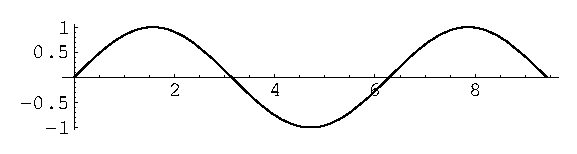
\includegraphics[width=8.5cm]{image1}}
%  \vspace{2.0cm}
  \centerline{(a) Result 1}\medskip
\end{minipage}
%
\begin{minipage}[b]{.48\linewidth}
  \centering
  \centerline{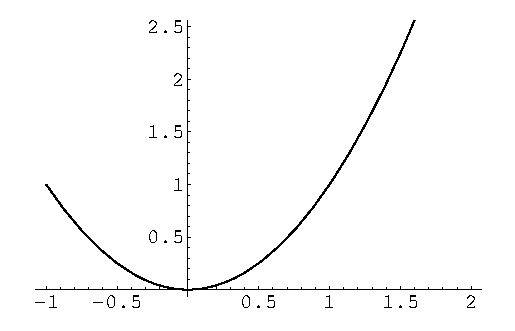
\includegraphics[width=4.0cm]{image3}}
%  \vspace{1.5cm}
  \centerline{(b) Results 3}\medskip
\end{minipage}
\hfill
\begin{minipage}[b]{0.48\linewidth}
  \centering
  \centerline{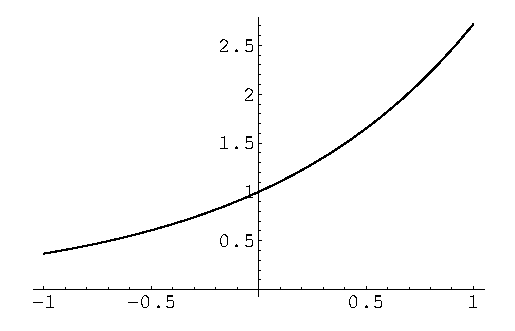
\includegraphics[width=4.0cm]{image4}}
%  \vspace{1.5cm}
  \centerline{(c) Result 4}\medskip
\end{minipage}
%
\caption{Example of placing a figure with experimental results.}
\label{fig:res}
%
\end{figure}


\vfill\pagebreak

\bibliographystyle{IEEEbib}
\bibliography{references}

\end{document}
